\documentclass[tikz,border=10pt]{standalone}
\begin{document}
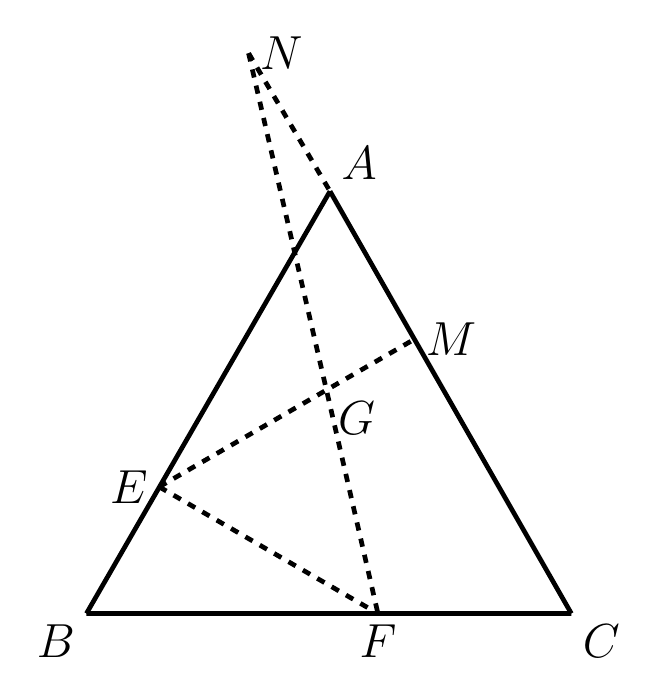
\begin{tikzpicture}[line width=1.7pt, line join=round]
\coordinate (A) at (0.008,2.018);
\coordinate (B) at (-3.085,-3.344);
\coordinate (C) at (3.073,-3.344);
\coordinate (F) at (0.617,-3.345);
\coordinate (G) at (-0.037,-0.506);
\coordinate (M) at (1.080,0.139);
\coordinate (N) at (-1.026,3.771);




\coordinate (E) at (-2.161,-1.736);


\draw[solid] (A)--(M)--(C);   
\draw[solid] (B)--(F)--(C);   
\draw[solid] (A)--(B);        


\draw[dashed] (N)--(A);

\draw[dashed] (N)--(G)--(F);

\draw[dashed] (E)--(G)--(M);

\draw[dashed] (E)--(F);


\node[above right] at (A) {\fontsize{17.5}{21}\selectfont $A$};
\node[right] at (N) {\fontsize{17.5}{21}\selectfont $N$};
\node[right] at (M) {\fontsize{17.5}{21}\selectfont $M$};
\node[below right] at (G) {\fontsize{17.5}{21}\selectfont $G$};
\node[left] at (E) {\fontsize{17.5}{21}\selectfont $E$};
\node[below left] at (B) {\fontsize{17.5}{21}\selectfont $B$};
\node[below] at (F) {\fontsize{17.5}{21}\selectfont $F$};
\node[below right] at (C) {\fontsize{17.5}{21}\selectfont $C$};
\end{tikzpicture}
\end{document}